\documentclass[a4paper,12pt]{scrartcl}
\usepackage[utf8x]{inputenc}
\usepackage[T1]{fontenc} % avec T1 comme option  d'encodage c'est ben mieux, surtout pour taper du français.
%\usepackage{lmodern,textcomp} % fortement conseillé pour les pdf. On peut mettre autre chose : kpfonts, fourier,...
\usepackage[french]{babel} %Sans ça les guillemets, amarchpo
\usepackage{amsmath}
\usepackage{multicol}
\usepackage{amssymb}
\usepackage{tkz-tab}
\usepackage{exercice_sheet}

%\trait
%\section*{}
%\exo{}
%\question{}
%\subquestion{}

\date{}


% Title Page
\title{Devoir en classe 1, OL-2, corrigé}

\author{Mathématiques}

\begin{document}

\maketitle

\exo{Résoudre les équations suivantes:}

\question{}
$2x^2 +4x - 2 = 0$

$\Delta = b^2 - 4ac = 32 > 0$. L'équation a donc 2 solutions.

$\sqrt{\Delta} = 4 \sqrt{2}$

$x_1 = \dfrac{-4-4\sqrt{2}}{4} = -1-\sqrt{2}$

$x_2 = \dfrac{-4+4\sqrt{2}}{4} = -1+\sqrt{2}$

L'ensemble des solutions $S$ s'écrit donc $S = \left\lbrace -1-\sqrt{2};-1+\sqrt{2} \right\rbrace$

\question{}
On pose $X = e^x$. L'équation devient donc:

$X^2 - 2X + 1 = 0$

$\Leftrightarrow (X - 1)^2 = 0$

$\Leftrightarrow X - 1 = 0$

$\Leftrightarrow X = 1$

$\Leftrightarrow e^x = 1$

$\Leftrightarrow x = 0$

$\Leftrightarrow x \in \left\lbrace 0 \right\rbrace$


\exo{Suites}

On place une somme d'argent notée $S_0$ au taux annuel de 5,5 \%, ce placement étant à intérêts composés.
Pour tout entier naturel $n$, $S_n$ désigne le capital disponible au bout de $n$ années.

\question{}
Justifier que la suite $(S_n)$ est géométrique. Préciser la raison $q$ de cette suite.

Chaque année, on ajoute 5.5\% de la valeur de l'année précédente. Ainsi, si $S_n$ est égal à la somme disponible l'année $n$, à l'année $n+1$ on aura $S_{n+1} = S_n + S_n \times 0.055 = 1.055 S_{n+1}$. 

On a donc $S_0 = 1.055$.

\question{}
Exprimer $S_n$ en fonction de $S_0$ et de $n$.

$S_n = S_0 \times q^n$

\question{}
$S_0 = 1500$ € en 2018. Quelle somme se trouvera sur le compte en 2029? Arrondir le résultat à l'euro près. 

L'année 2029 correspond au rang $n=11$. On a donc $S_{11} = S_0 \times q^{11} = 1500 \times 1.055^{11} = 2703$€.

\exo{Statistiques à deux variables}

Pour les besoins d'une usine qui fabrique des puces, l'entreprise TERRARE extrait du minerai rare. Sa production annuelle $X$ (en
tonnes) n'excède pas 2 tonnes et le coût total annuel de la production est noté $Y$ en milliers d'euros (1 k€ = 1000 €).
Les résultats des premières années d'exploitation sont consignés dans le tableau suivant:

\begin{table}[h]
\centering
\caption{}
\label{tableau_2}
\begin{tabular}{|l|l|l|l|l|l|}
\hline
année          & 2006  & 2007  & 2008  & 2009  & 2010  \\ \hline
$x_i$ (tonnes) & 0.52  & 0.77  & 1.01  & 1.36  & 1.81  \\ \hline
$y_i$ (k€)     & 186.7 & 230.9 & 283.1 & 381.3 & 558.9 \\ \hline
$z_i$&5.230&5.442&5.646&5.944&6.326 \\ \hline
\end{tabular}
\end{table}

\question{}
Le plan est muni d'un repère orthogonal.
Unités graphiques : 1 cm pour 0,1 unité sur l'axe des abscisses et 2 cm pour 100 unités sur l'axe des ordonnées.
Construire le nuage de points associé à cette série statistique sur votre copie. 

\begin{center}
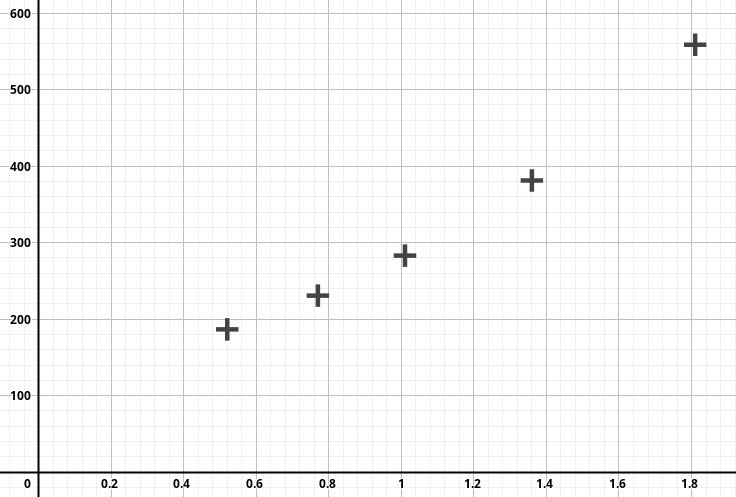
\includegraphics[width=0.7\textwidth]{graph.png}
\end{center}

\question{}
La nature de l'activité et le graphique laissent penser qu'un ajustement exponentiel est approprié. On pose $z = \ln y$.

\subquestion{}
Compléter le tableau ci-dessus.
Arrondir à $10^{-3}$ les valeurs de $z_i$.

\subquestion{}
Déterminer le coefficient de corrélation linéaire $r$ entre $x$ et $z$. Arrondir à $10^{-3}$.

En arrondissant, on trouve 1.000.

\subquestion{}\label{question}
À l'aide de la calculatrice, déterminer par la méthode des moindres carrés, une équation de la droite d'ajustement de $z$
en $x$. Les coefficients seront arrondis à $10^{-2}$.

$a = 0.85$

$b = 4.79$

On peut donc écrire $z = 0.85x + 4.79$

\question{}
Estimations.

\subquestion{}
Déduire de la question précédente une expression de $y$ en fonction de $x$, de la forme $y = B \cdot e^{ax}$ où $a$ est un réel et où $B$ sera arrondi à l'entier le plus proche.

$z = \ln y \Leftrightarrow y = e^z$

Soit $y = e^{0.85x + 4.79} =  e^{4.79} \times e^{0.85x} \approx 120 \cdot e^{0.85x}$.

On a donc bien la forme $B \cdot e^{ax}$ avec $B = 120$ et $a = 0.85$

\subquestion{}
En déduire une estimation du coût de production pour 2 tonnes.

Estimation de $y$ pour $x = 2$. 

$y = 120 e^{0.85 \times 2} \approx 657$K€.

\exo{Loi normale}%Exercice 1 partie B ci-joint

 Une usine fabrique des billes de diamètre 8mm. Les erreurs d'usinage provoquent des variations de diamètre. On estime, sur les données antérieures, que l'erreur est une variable aléatoire qui obéit à une loi normale de paramètres $\mathcal{N}(8;0.02)$.

On tire une bille produite par cette usine au hasard.

\question{}
On trouve $P(X \geqslant 8.5) \approx 0$.

\question{}
La probabilité qu'une bille soit prise au hasard soit retenue est $P(7.97 \geqslant X \geqslant 8.03) = 0.866$. 

La probabilité qu'elle soit rejetée est donc $1 - P(7.97 \geqslant X \geqslant 8.03) = 0.134 = 13.4$ \%

\trait

\begin{center}
Fin.
\end{center}

\end{document}
